% gold_letter.tex
%
% A policy letter in the format of a Chicago Fed Letter: roughly 3,400 words,
% four figures, declarative section headings, endnotes.
%
% NOT a Federal Reserve publication and deliberately not dressed as one. No
% masthead, issue number, DOI or institutional disclaimer, because those would
% present it as something it is not. The genre is borrowed; the institution is
% not.
%
% Build (two passes, for the endnote numbering):
%   pdflatex -interaction=nonstopmode gold_letter.tex
%   pdflatex -interaction=nonstopmode gold_letter.tex
%
% latexmk is avoided on this machine: MiKTeX exits non-zero on an unsupported
% Windows build even when the PDF is fine.

\documentclass[11pt]{article}

\usepackage[letterpaper,margin=1.05in,top=1.0in,bottom=1.1in]{geometry}
\usepackage[T1]{fontenc}
\usepackage[utf8]{inputenc}
\usepackage{charter}
\usepackage[scaled=0.92]{helvet}
\usepackage{graphicx}
\usepackage{booktabs}
\usepackage{enumitem}
\usepackage{endnotes}
\usepackage{caption}
\usepackage{microtype}
\usepackage[hidelinks]{hyperref}
\usepackage{xcolor}

\definecolor{ink}{HTML}{121212}
\definecolor{soft}{HTML}{555555}
\definecolor{rule}{HTML}{BBBBBB}

\usepackage{titlesec}
\titleformat{\section}{\sffamily\bfseries\large\color{ink}}{}{0pt}{}
\titlespacing*{\section}{0pt}{16pt}{6pt}

\captionsetup[figure]{labelformat=empty, justification=raggedright,
  singlelinecheck=false, font={sf,small}, skip=6pt}

\setlength{\parskip}{6pt}
\setlength{\parindent}{0pt}
\renewcommand{\baselinestretch}{1.06}

% Endnotes, numbered, set small at the end under a plain heading.
\renewcommand{\enotesize}{\small}
\renewcommand\enoteheading{\section*{\sffamily\bfseries\large Notes}}

\newcommand{\fignote}[2]{%
  \par\vspace{2pt}{\sffamily\footnotesize\color{soft}%
  \textbf{Notes:} #1\par\textbf{Sources:} #2\par}}

\begin{document}
\pagestyle{empty}

% ------------------------------------------------------------------ masthead
{\sffamily\footnotesize\color{soft} ECONOMIC RESEARCH NOTE \hfill September 2026}

\vspace{4pt}
{\color{rule}\hrule height 2pt}
\vspace{10pt}

{\sffamily\bfseries\LARGE\color{ink}
When gold moves but trade does not:\\ nonmonetary gold in the U.S. trade statistics\par}

\vspace{6pt}
{\sffamily\small\color{soft} Samuel Moore\par}

\vspace{10pt}

% ------------------------------------------------------------------ abstract
{\sffamily\small\color{ink}
Between December 2024 and March 2025 the United States imported roughly 870
tonnes of gold more than its own decade-long trend implies --- about a quarter
of annual world mine production --- and by mid-2026 most of it had gone back
out again. This letter shows that the episode was a change of address rather
than a change in trade. The metal moved when, and only when, the price of gold
\emph{in New York} rose far enough above the price of gold \emph{in London} to
cover the cost of flying it across the Atlantic. That cost turns out to be very
small: the whole round trip consumed an estimated \$243 million of real
resources, 0.14\% of the \$174 billion of metal it shuttled. The measurement
consequences were not small. Gold accounts for 26\% of the record January 2025
trade deficit and 41\% of the unusually narrow October 2025 figure, and the
twelve-month deficit was overstated by \$79 billion at its peak. The national
accounts already exclude nonmonetary gold for precisely this reason. The trade
release does not, and we argue it should.\par}

\vspace{12pt}
{\color{rule}\hrule height 0.5pt}
\vspace{6pt}

% ------------------------------------------------------------------ body
Gold is an awkward object for a trade statistician. Most of what crosses a
border does so because somebody intends to consume it, install it, or turn it
into something else. Gold bullion frequently crosses a border for none of those
reasons. It moves because its owner wants it held somewhere else --- in a
different vault, under a different legal wrapper, in a different
jurisdiction --- while remaining, economically, the same asset belonging to the
same person. Nothing has been produced and nothing has been consumed. An address
has changed.

Customs authorities record the crossing all the same, because a crossing is what
they are built to observe. In ordinary times this matters little: monthly U.S.
imports of nonmonetary gold ran between one and four billion dollars for most of
the past decade, a rounding error against goods imports of roughly \$270 billion
a month. Between December 2024 and March 2025 they did not. Imports reached
\$34.2 billion in January 2025 alone,\endnote{Combining Harmonized System
headings 7108 and 7115; see note 3.} and the three largest monthly U.S. trade
deficits in the history of the series --- which begins in 1992 --- fall
consecutively in that window.

This letter asks what happened, what it cost, and what it did to the published
numbers. We take no position on the trade policy that set it off. The trigger is
treated here purely as a date after which the expected tariff treatment of gold
imports became uncertain, and the question is what the statistical system did
with the flow that followed.

\section{Gold behaved like nothing else in the trade data}

Figure 1 places gold among the goods the United States actually trades. Each
point is one product or one partner, positioned by average monthly exports and
imports on logarithmic axes, in three phases: a baseline year, the five-month
surge, and the reversal that followed. Above the diagonal the United States is a
net importer of that item; below it, a net exporter. A commodity whose trade
grows normally drifts outward along the diagonal. A commodity the United States
starts buying moves up.

Gold does something else entirely. It moves sharply up and to the left into the
surge --- imports multiplying while exports fall --- and then travels back down
and to the right, ending the reversal phase further from the diagonal on the
export side than where it began. Switzerland, in the right-hand panel, traces
the same shape for the same reason: it is where the bars are recast into the
sizes the New York exchange accepts.\endnote{COMEX gold contracts settle against
100-ounce and kilobar deliverable forms. The London market trades 400-ounce Good
Delivery bars. Metal moving between the two therefore passes through a Swiss
refinery, which is why a bilateral U.S.--Switzerland series picks up so much of
this.} Of the 100 most-traded headings, no other traces an out-and-back path of
remotely this size.

That shape is the first piece of evidence, and it is worth being precise about
why. Metal that has been absorbed --- fabricated into jewellery, bought as a
retail coin, consumed in electronics --- does not come back. Metal that has been
relocated does, as soon as the reason for relocating it disappears. A round trip
in the trade data is the signature of relocation, and it is not a signature that
ordinary imports produce.

\begin{figure}[htbp]
\centering
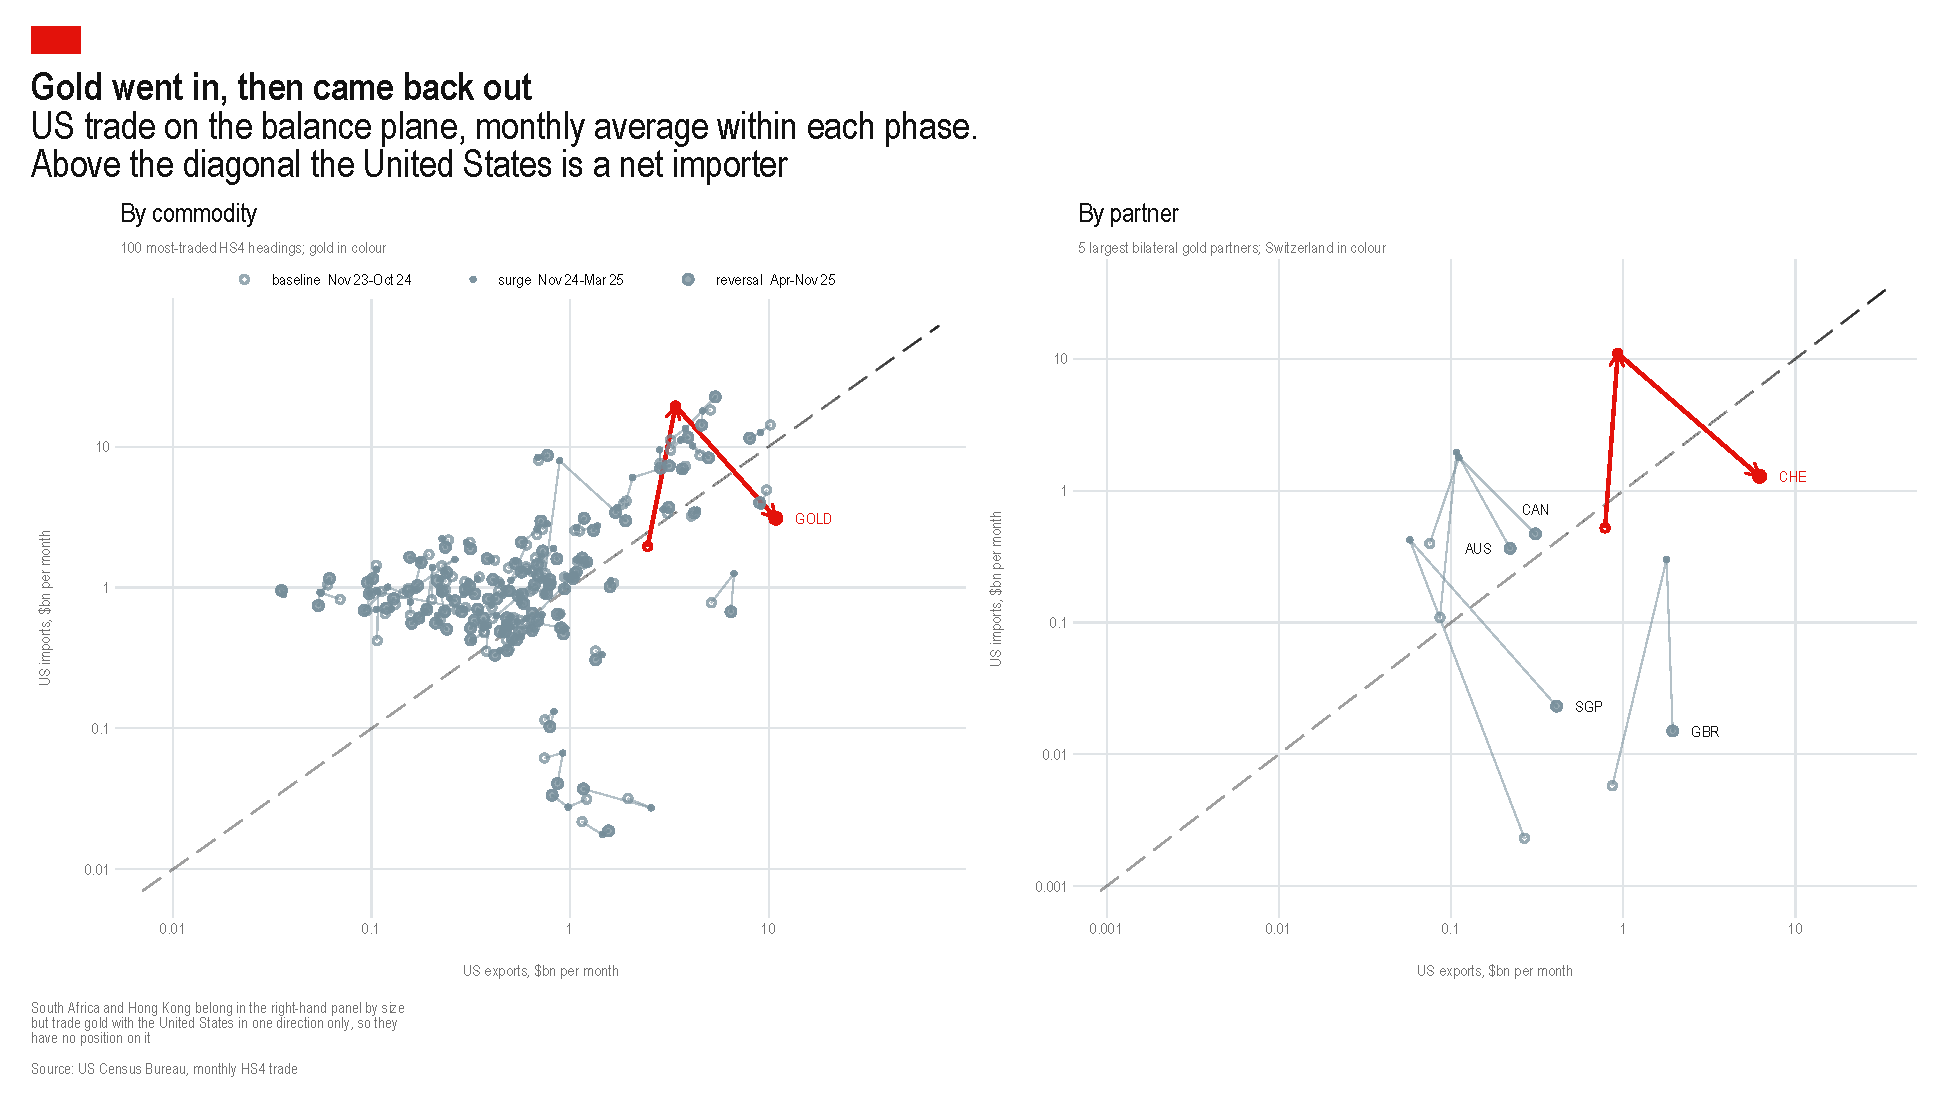
\includegraphics[width=\textwidth]{../figures/gold_panel.pdf}
\caption{\textbf{1. U.S. trade on the balance plane, by commodity and partner,
November 2023--November 2025}}
\fignote{Each point is the monthly average within a phase, so that phases of
different length are comparable. Both axes are logarithmic, so a series must
trade in both directions in all three phases to appear. Gold combines HS 7108
and 7115.}{U.S. Census Bureau.}
\end{figure}

\section{The price of location, not the price of gold}

If the metal moved for a reason, the reason should be visible in a price. It is,
but not in the price of gold. It is in the difference between the price of gold
in two places.

The relevant object is familiar to any international economist under a different
name. Covered interest parity says that the forward premium on a currency must
equal the interest differential, or a riskless arbitrage exists. Gold obeys the
same logic with the interest rate replaced by the cost of storing metal:

\begin{quote}
$F(\tau) = S \cdot e^{b\tau}$,
\end{quote}

where $S$ is the spot price, $F(\tau)$ the futures price for delivery $\tau$
days out, and $b$ the cost of carrying an ounce for a day --- financing, storage
and insurance, net of any income from lending the metal out. If the futures
curve satisfies this relation, a gold futures contract is a claim on the same
metal at a later date, and nothing more.

It need not. Deliverable futures are claims on metal \emph{in a particular
place}. A COMEX contract delivers in New York; the London benchmark prices metal
in London. When the two diverge by more than carry, the gap is not compensation
for time. It is the price of location.

We estimate that price directly. Each trading day we project the whole COMEX
futures curve onto a line in log price against days to delivery, weighting each
contract by its open interest:
\begin{quote}
$\ln F_i(\tau_i) = a + b\,\tau_i + u_i$.
\end{quote}
The slope $b$ is the carry. The intercept $a$ is what the curve implies New York
gold is worth for immediate delivery, and the premium is that intercept over the
London price, $p = a - \ln S$. This is a reduced form: $p$ is defined by the
projection, and we make no attempt to split it into its location, form and trust
components, which we do not believe are separately identified.

One correction matters more than it sounds. The COMEX settlement is struck at
13:30 in New York and the London benchmark at 15:00 in London --- three and a
half hours apart, or two and a half for the three weeks each year when one
country has changed its clocks and the other has not. Gold moves in that gap,
and the movement enters $p$ as pure measurement error. Because it is common to
every contract on a given day, it lands entirely on the intercept and not at all
on the slope, so it can be removed by pricing both legs at the same instant from
minute data. Doing so cuts the standard deviation of the daily premium from
0.499\% to 0.235\%. More than half the apparent day-to-day variation in the
spread was an artifact of comparing two prices struck at different times.

Figure 2 plots the result against what an arbitrageur must clear: the carry to
delivery plus the one-off cost of flying and recasting an ounce. Below that
band, moving metal loses money and nothing should move. Above it, the trade
pays.

The lower panel shows what did move. Over 2,862 trading days the spread cleared
the westward threshold on 835 and the eastward one on 1,169 --- normally the
United States is a net \emph{exporter} of gold, and for most of the sample the
spread sits where that is the profitable direction. In the episode both series
move together: the premium rises, and 867 tonnes go west on net between December
2024 and March 2025. From April 2025, once gold was excluded from the announced
tariff schedule and the premium fell back through the band, 281 tonnes come
back.

The relationship is not mechanical, and the figure is honest about that. The
spread cleared the cost of shipping in many months when very little metal moved.
Clearing the threshold makes a shipment profitable; it does not compel one. What
the figure establishes is the weaker but sufficient claim: the metal moved when
the price of location made it worth moving, and in the direction that price
pointed.

\begin{figure}[htbp]
\centering
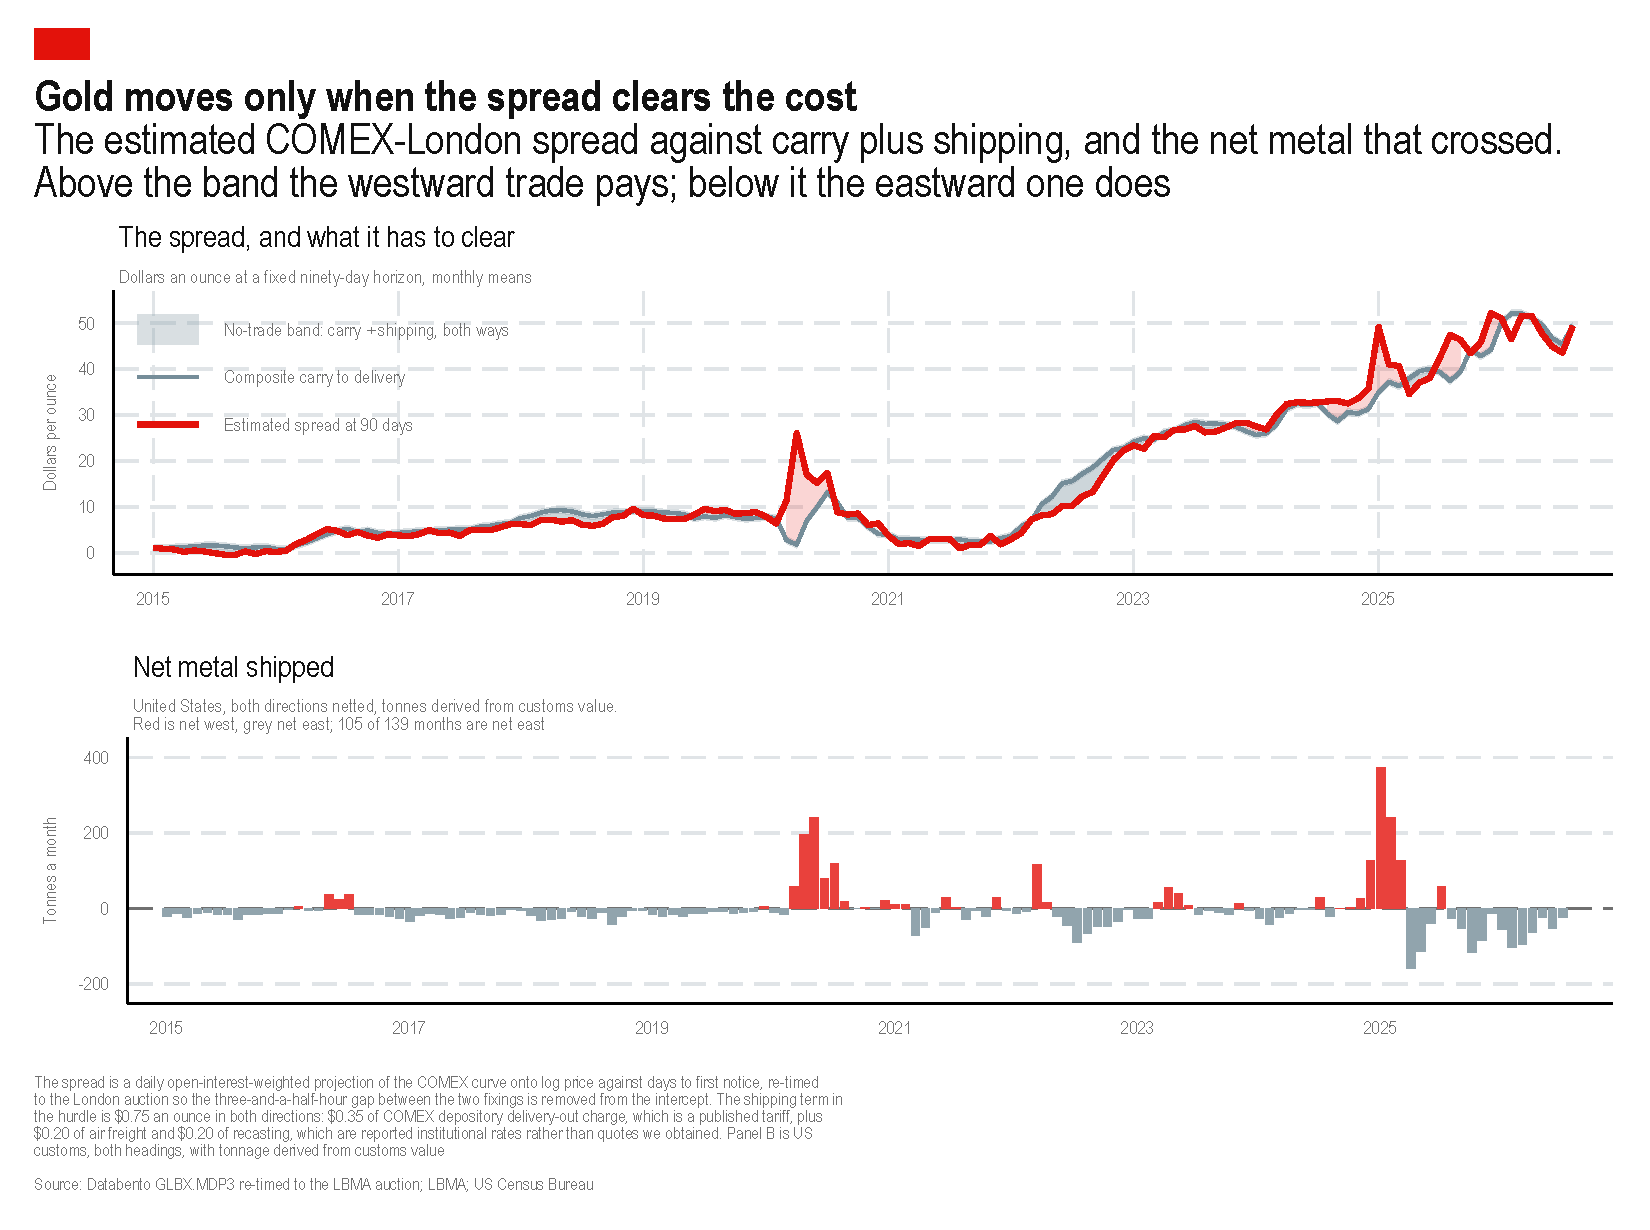
\includegraphics[width=\textwidth]{../figures/spread_vs_hurdle.pdf}
\caption{\textbf{2. The COMEX--London spread against the cost of moving metal,
and the net flow, 2015--2026}}
\fignote{The spread is a daily open-interest-weighted projection of the COMEX
curve onto log price against days to first notice, re-timed to the London
auction. The shipping component of the hurdle is \$0.75 an ounce in both
directions, of which \$0.35 is the published COMEX depository delivery-out
charge. Tonnage in the lower panel is derived by dividing customs value by the
London benchmark.}{Databento (CME Globex MDP 3.0); LBMA; CME Group; U.S. Census
Bureau.}
\end{figure}

\section{About 870 tonnes crossed that otherwise would not have}

How much of the flow was the episode, and how much was the trade that would have
happened anyway? Figure 3 answers this in the simplest available way. We fit a
straight line by least squares to all 118 months of U.S. gold imports from
January 2015 to October 2024, carry it forward unchanged, and measure the area
between the actual series and that line.

The pre-period is deliberately the whole of it rather than a recent slice. A
short window invites the objection that it was chosen to flatter the result; a
decade does not, and the fitted line is drawn across the entire chart so the
reader can judge the fit against the data that produced it. The line rises at
0.090 tonnes a month --- U.S. gold imports were very gently trending up --- and
reaches 41 tonnes by January 2025 against an actual figure nine times larger.

The five-month episode runs \textbf{873 tonnes} above the line. Over the whole
21 months since the break, and netting off the fifteen months that fall
\emph{below} it, the excess is 540 tonnes. For scale, the episode figure is
about a quarter of annual world mine production. It is a great deal of metal to
move for a reason unrelated to anybody wanting to own more of it.

Two caveats belong with that number. It is a difference from an extrapolated
line, not a causal estimate: anything else moving gold westward in those months
is counted here as episode excess. And because U.S. customs data report value
rather than weight for these headings, the tonnage is derived by dividing by the
London benchmark, which makes it a slightly different measurement from the
Swiss and British export figures that carry mass directly.

\begin{figure}[htbp]
\centering
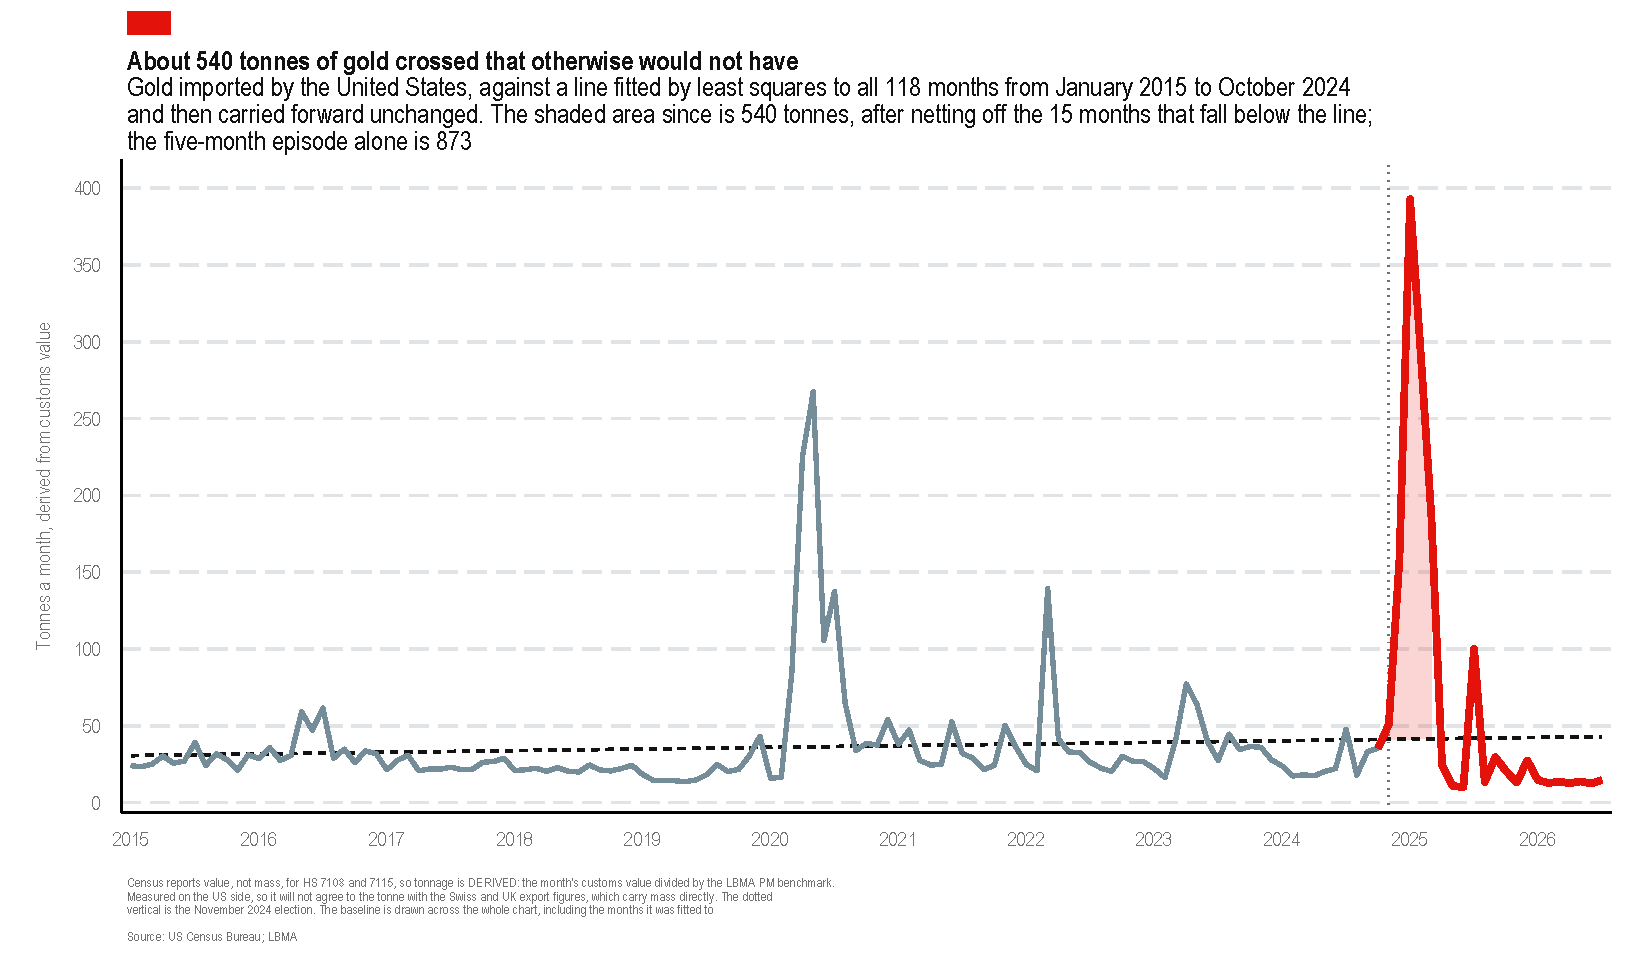
\includegraphics[width=\textwidth]{../figures/counterfactual.pdf}
\caption{\textbf{3. U.S. gold imports against a pre-episode trend, 2015--2026}}
\fignote{The baseline is a least-squares line fitted to all 118 months before
November 2024 and carried forward unchanged; it is not clipped, and it is drawn
across the months it was fitted to as well as the months it projects. Tonnage is
derived from customs value at the London benchmark.}{U.S. Census Bureau;
LBMA.}
\end{figure}

\section{Moving it was remarkably cheap}

What did the relocation consume? The question is worth asking precisely, because
it is the one place where a reassuring answer is the correct one.

Freight is charged by weight, recasting by the bar, and exchange handling by the
ounce, so those three are fixed dollar amounts that do not move with the gold
price. Insurance and the financing of metal in transit are charged on value, so
they roughly doubled over this sample because gold did. Adding them gives an
all-in cost of \$1.70 to \$10.72 an ounce for one leg, with a central estimate
near \$4.94.\endnote{The freight, recasting and handling components are built up
separately in figure 2's hurdle, where they total \$0.75 an ounce: \$0.35 of
published COMEX depository delivery-out charge --- \$35.00 per 100-ounce
contract, with delivery in free --- plus \$0.20 of air freight and \$0.20 of
recasting at the institutional rates reported during the episode. The wider
range quoted here adds insurance and transit financing, which scale with the
gold price and therefore roughly doubled over this sample. We did not obtain
carrier quotes; a single one would be the cheapest available improvement to
both figures. Retail parcel rates of \$300--500 a kilogram circulate widely and
are not used: they price a one-kilo consignment to a private buyer rather than a
tonne moving between bullion banks, and are two orders of magnitude too high.}

Applying that to the excess metal in both directions --- 1,632 tonne-legs, since
a round trip is two flights and two recastings --- gives a bill of
\textbf{\$243 million}, with a range of \$85 million to \$520 million. Set
against the \$174 billion of metal those legs carried, that is
\textbf{0.14\% of the value moved}.

This is the central fact about the episode's real consequences, and it cuts in
an unglamorous direction. Relocating gold is close to free relative to what gold
is worth. That is precisely why a few dollars an ounce of price differential was
able to move a quarter of a year's mine output in five months: the barrier to
moving it was never high. It also means the episode destroyed very little. No
factory was idled and no consumer went without. Roughly a quarter of a billion
dollars of freight, insurance, refining and financing was consumed to move metal
into a vault it subsequently left --- wasteful in the narrow sense, and trivial
in any aggregate sense.

The consequences that are \emph{not} trivial are informational.

\section{What it did to the published trade figures}

Figure 4 puts the monthly U.S. goods-and-services deficit next to the same
balance with nonmonetary gold removed from both sides. The adjustment is one
line of arithmetic: the published balance is exports minus imports, so taking
gold out of both gives the balance plus net gold imports. We subtract it
\emph{from} the published series rather than rebuilding a deficit from scratch,
so the two lines differ by the gold and by nothing else.

The gap is large exactly when the headline was most discussed. January 2025
printed a record \$124.7 billion deficit; without the gold it is \$92.2 billion,
so \textbf{26\% of the record was bullion}. October 2025 printed \$37.4 billion,
the narrowest in six years and widely read as an improvement in the trade
position; without the gold it is \$52.6 billion, so \textbf{41\% of the
improvement was bullion leaving the country}. The same mechanism produced three
consecutive record deficits and, seven months later, the best trade month in six
years. Neither was trade in any economically meaningful sense.

The natural reassurance is that a round trip nets out over a year and only the
monthly print is affected. That reassurance is wrong, and it is worth stating
plainly because it is the first thing most readers will reach for. At its March
2025 peak the rolling twelve-month deficit was overstated by \textbf{\$79.5
billion}, 7.4\% of the trailing-year total, because a full year of data then
contained the entire surge and none of the reversal. Eleven months after the
metal began moving, the twelve-month figure was still overstated by \$16 billion.
The distortion is slower than the annual frequency at which most people read
trade data.

\begin{figure}[htbp]
\centering
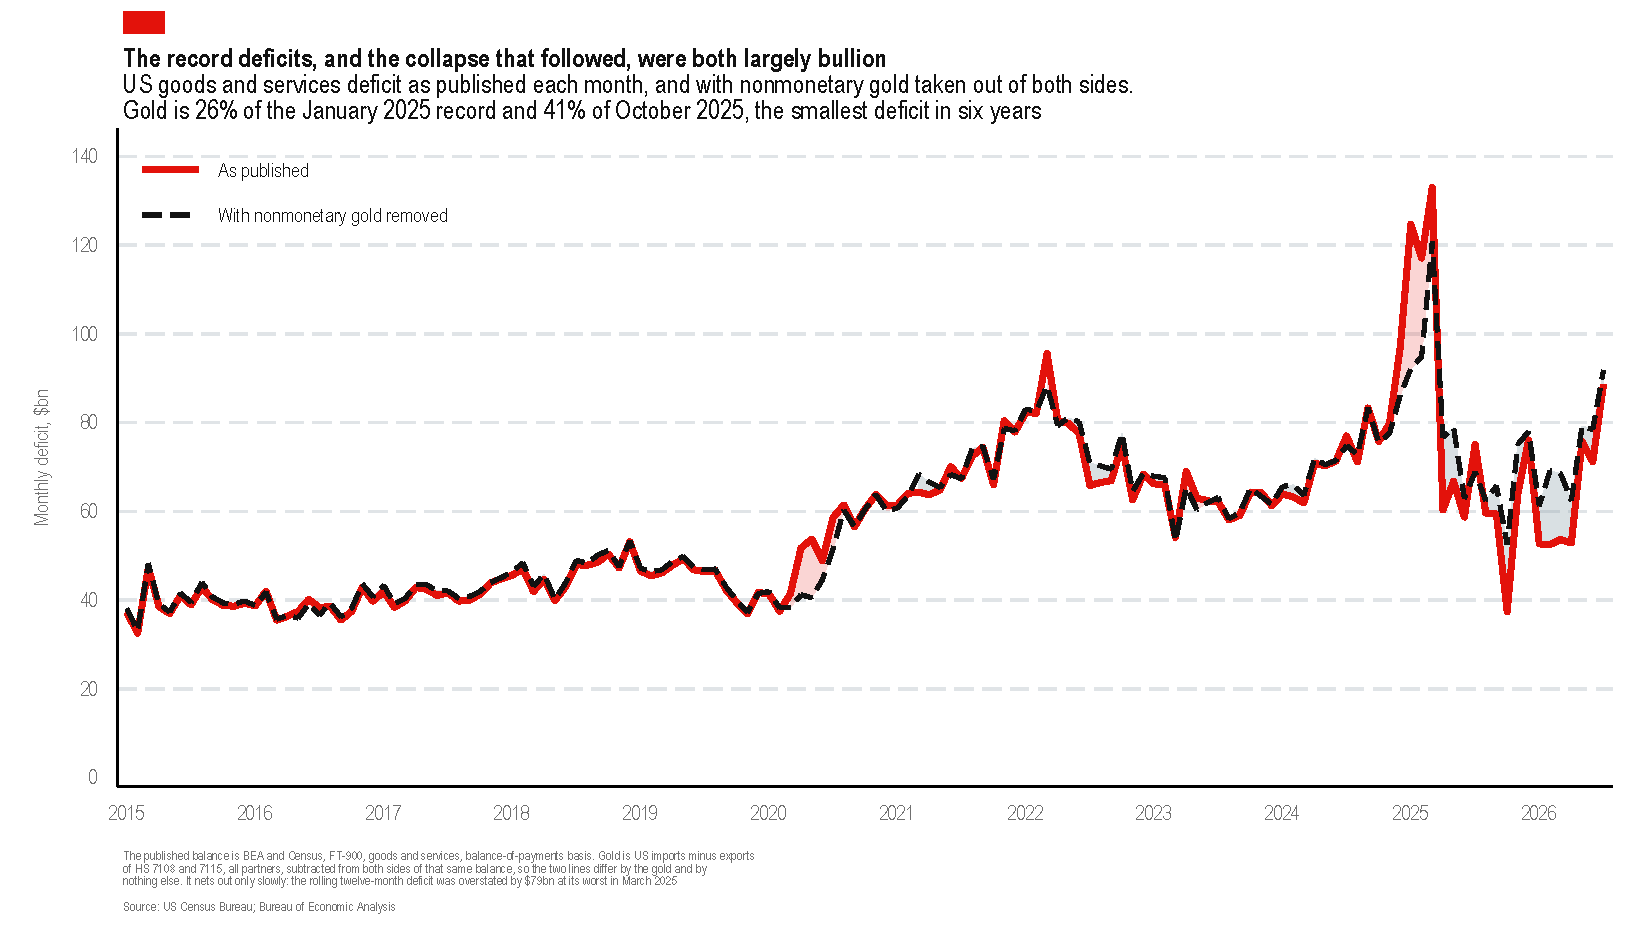
\includegraphics[width=\textwidth]{../figures/deficit_gold.pdf}
\caption{\textbf{4. The U.S. monthly trade deficit as published and with
nonmonetary gold removed, 2015--2026}}
\fignote{Gold is U.S. imports minus exports of HS 7108 and 7115, all partners,
subtracted from both sides of the published balance. Shading is red where gold
widened the deficit and grey where it narrowed it; the deficit is plotted as a
positive number, so up is wider.}{U.S. Census Bureau; Bureau of Economic
Analysis.}
\end{figure}

\section{The national accounts already make this adjustment}

There is a straightforward precedent for what we are suggesting, and it is
already in force one department away.

The Bureau of Economic Analysis does not allow nonmonetary gold into the
national accounts. Its stated treatment is to \emph{remove} exports and imports
of nonmonetary gold from the international transactions data and replace them
with an adjustment computed as domestic production less industrial use.\endnote{%
See BEA, ``How are exports and imports of nonmonetary gold treated in BEA's
National Economic Accounts?'', and the NIPA Handbook, chapter 8, with the
reconciliation in table 4.3C.} The reasoning is exactly the reasoning of this
letter: a bar bought as a store of value is a \emph{valuable}, not consumption
and not investment, so admitting it to gross domestic product would record
activity that did not occur. This is long-standing practice, not a response to
2025.

That the rule is live rather than nominal can be seen in what BEA did with a
neighbouring metal. In the first quarter of 2025 it identified and removed a
surge in imports of silver bars from industrial supplies and materials, because
silver bars arrive under a heading the standing gold adjustment does not reach.
Gold required no mention because gold comes out as a matter of course.

The trade release applies no such filter. The consequence is that the same metal
is excluded from one official statistic and headlined in another, and a reader
who moves between the two has no way to see it from the published figures.

The cost of that gap was borne, visibly, by forecasters. A nowcasting model
bridges from monthly trade data to a quarterly GDP concept; if the trade series
contains gold and the GDP concept excludes it, the bridge is mapping one thing
onto another. In early March 2025 the Federal Reserve Bank of Atlanta
recalibrated its GDPNow model to strip gold out of the trade aggregates it
extrapolates from, ran the standard and gold-adjusted versions side by side for
two months, and on 30 April made the gold-adjusted version the standard
model.\endnote{Federal Reserve Bank of Atlanta, ``Adjustments for Gold Imports
and Exports in Standard GDPNow Model.'' Over the two months both models ran, the
gap between them was about two percentage points of annualized growth.} A
respected model had to be rebuilt mid-quarter because a published series
measured something its target did not.

\section{Conclusion}

The 2025 gold episode is a clean case of a general problem. Trade statistics
record border crossings, and a border crossing is an excellent proxy for
economic activity right up until the moment it is not. For most goods the proxy
holds. For bullion held as a store of value it fails completely: the metal
crosses, the statistic registers, and nothing has been produced, consumed or
even, in the relevant sense, traded.

The episode was cheap in resources and expensive in information. Roughly
\$243 million of freight, insurance, recasting and financing --- 0.14\% of the
value shuttled --- bought a distortion that accounted for a quarter of a record
monthly deficit, two-fifths of an unusually narrow one, and \$79 billion of a
trailing-year figure.

The remedy does not require a new concept, only the consistent application of an
existing one. BEA already computes the nonmonetary gold adjustment for the
national accounts, and the underlying series are already collected. Publishing
the goods balance on both bases --- as reported, and excluding nonmonetary
gold --- would let users see the wedge at the moment they read the headline
rather than reconstructing it afterwards from a classification detail.

Two features of the data make this more than a presentational nicety. Most of
the surge entered the United States under HS 7115, ``articles of precious
metal,'' rather than the heading one would search first; a user pulling HS 7108
alone would have found almost none of the episode.\endnote{BEA reclassifies
line 7115900530 --- rectangular shapes, 99.5\% or more gold, not otherwise
decorated --- as nonmonetary gold on a balance-of-payments basis, while the
Census classification treats it as a finished metal shape. The two agencies
disagree about what this metal is, which is why a Census-basis pull must add
7115 back by hand.} And the distortion does not wash out at annual frequency, so
waiting does not solve it.

None of this is a claim that any published number was wrong. The gold crossed
the border, and the balance of payments is designed to record goods crossing
borders. The claim is narrower: for this particular good, in these particular
quantities, the crossing and the economics came apart, and the statistical
system already knows how to tell them apart when it chooses to.

\vspace{8pt}
{\color{rule}\hrule height 0.5pt}
\vspace{4pt}

{\sffamily\footnotesize\color{soft}
All estimates in this letter are reproducible from public data and one
commercial futures feed. The pull scripts, the analysis and the code for each
figure are available in the project repository.\par}

\theendnotes

\end{document}
